\section{Evaluation}
	In this section, several sets of experiments are conducted to evaluate clustering algorithms. We compare the effects of the proposed method with three other methods including traditional MST(like Prim's or Kruscal's) algorithm, FMST\cite{zhong2015} and PNNG\cite{Jothi2018}. 

	We implement all our algorithms in Python. All the experiments were performed on a computer with Intel(R) Corel(TM) 3.2GHz i5-3470 CPU and 4 GB RAM. The operating system is Windows 7. The source code for Zhong-MST is from the original author and the source code for k-means and spectral clustering are from the python package.
	\subsection{Results on synthetic datasets}
		We select 8 synthetic datasets. The results are shown in Figure 4 and Figure 5.
% 二维数据集 MST结果展示  和标准MST的对比
% 边的数量和权重
	
		\begin{figure}[!t]
	        \centering
	        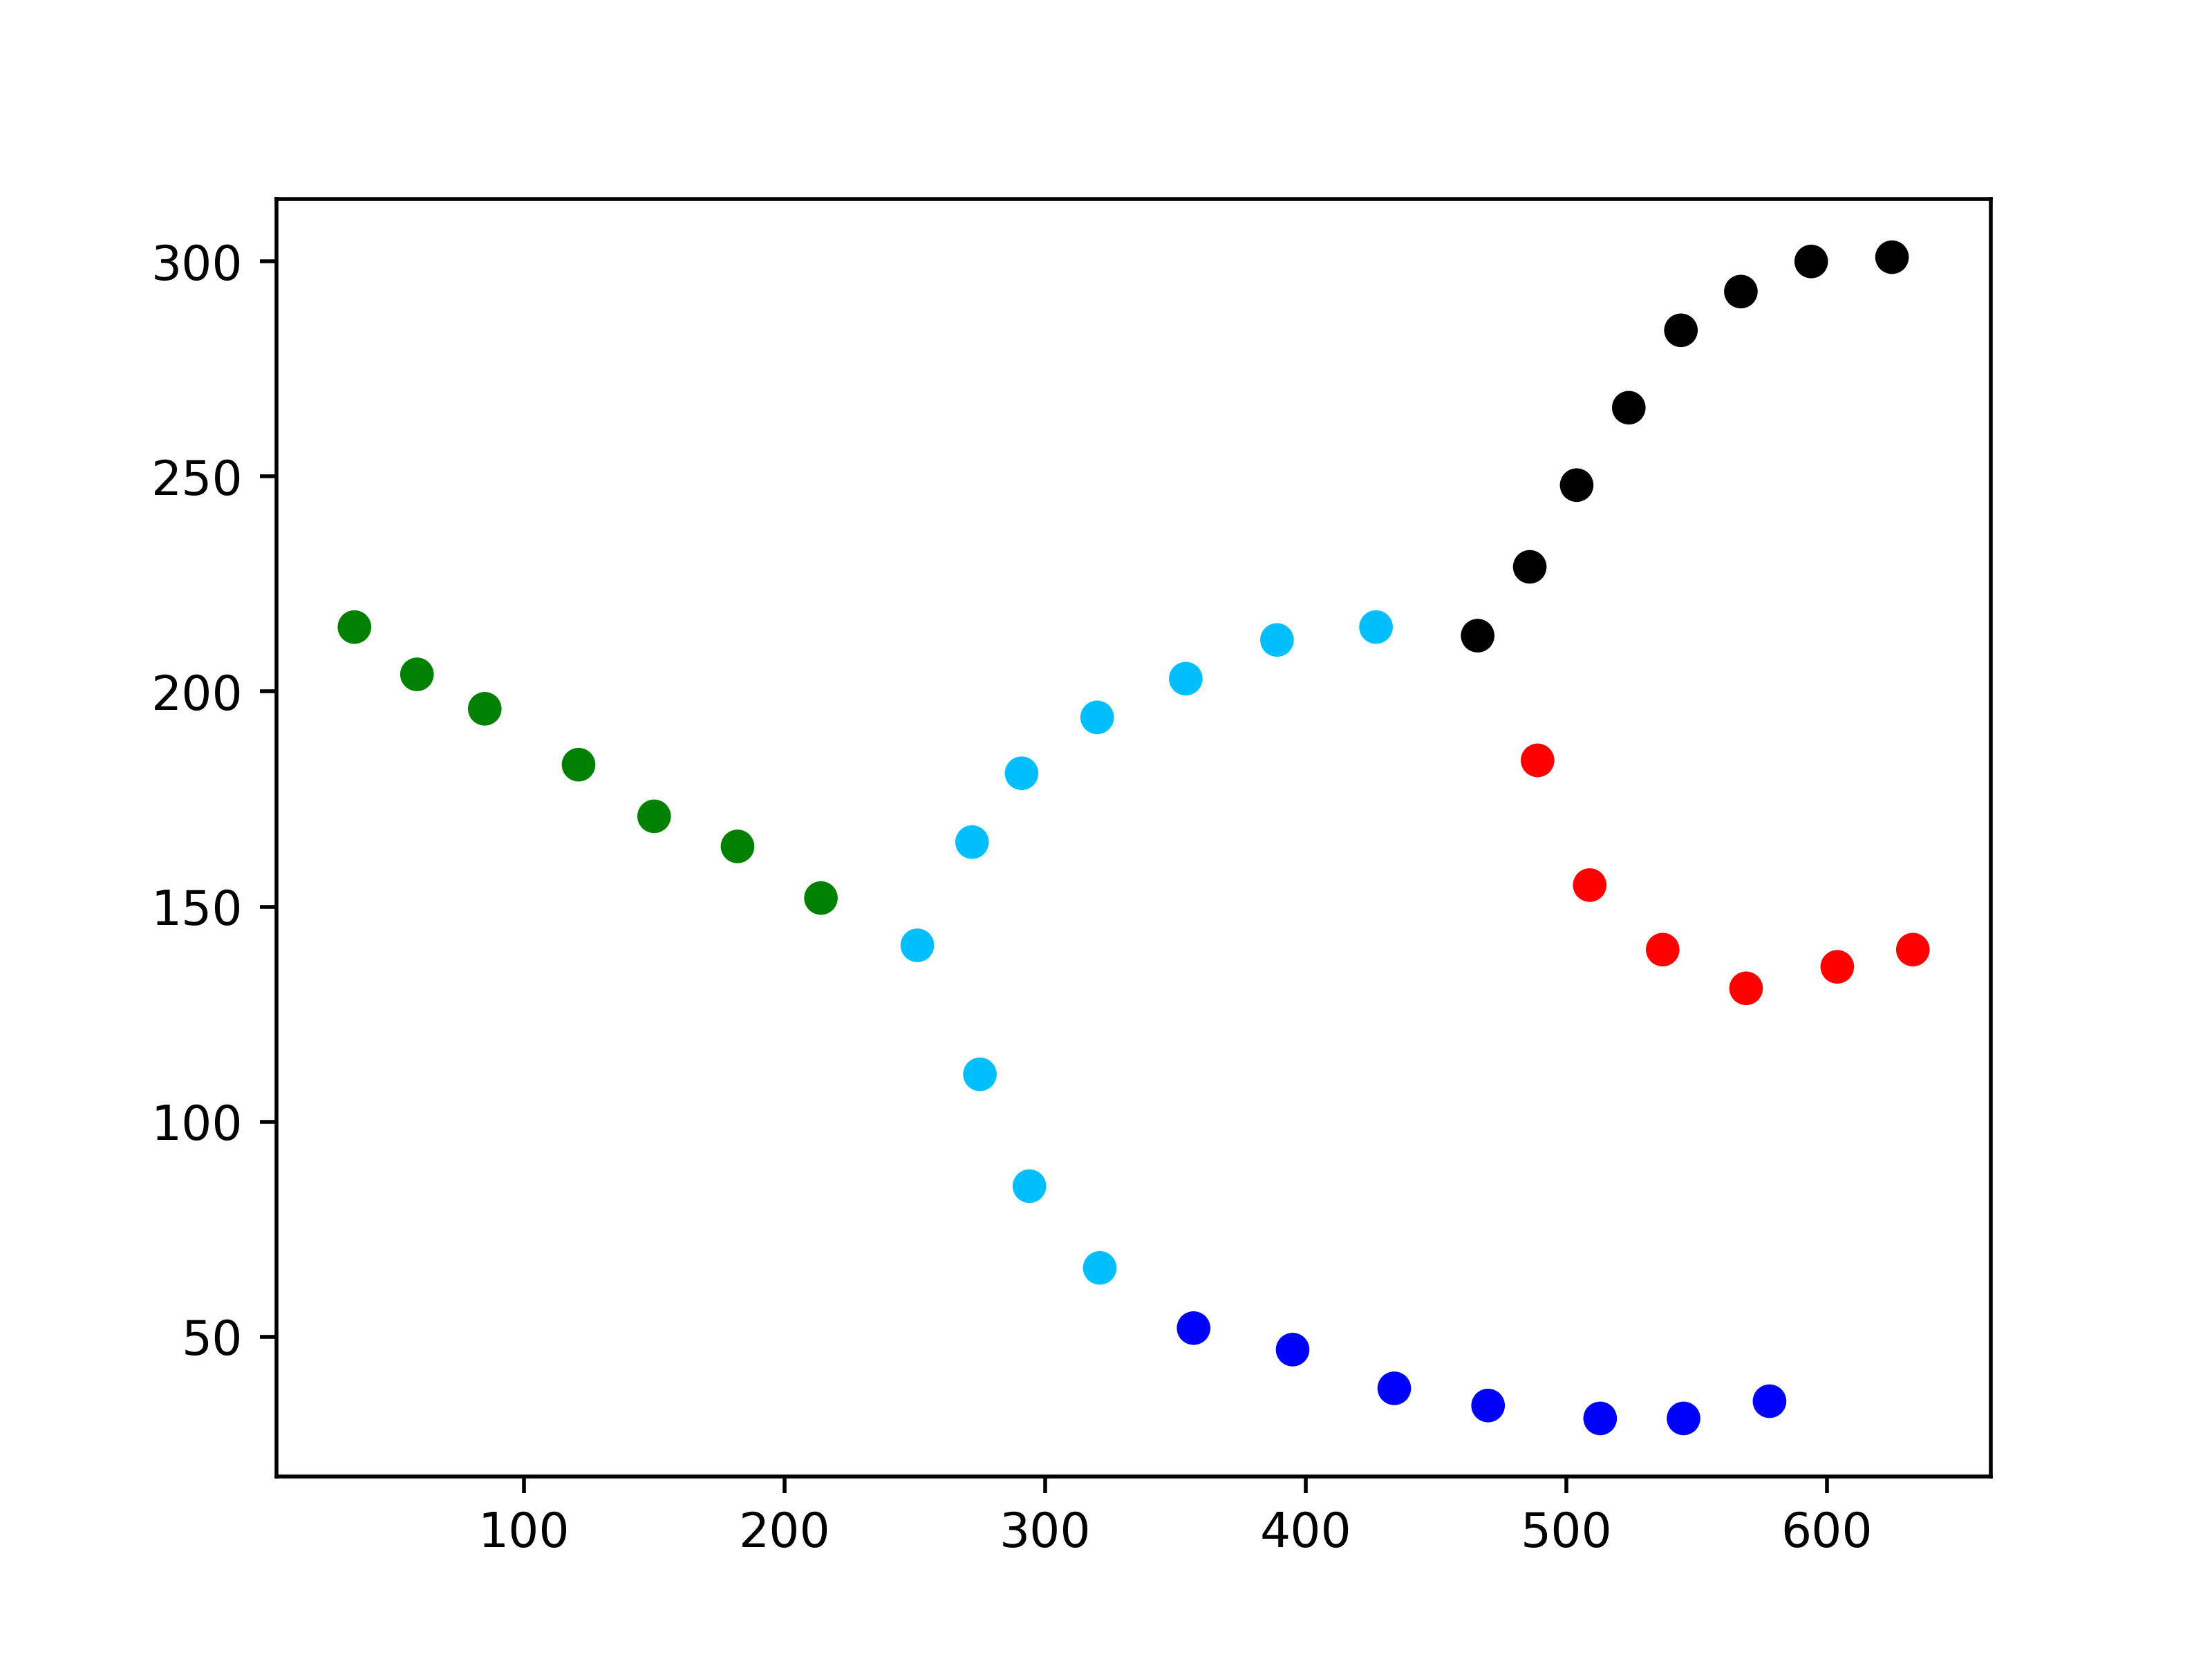
\includegraphics[width=0.43\linewidth]{our_density_d_clusters.png}
	        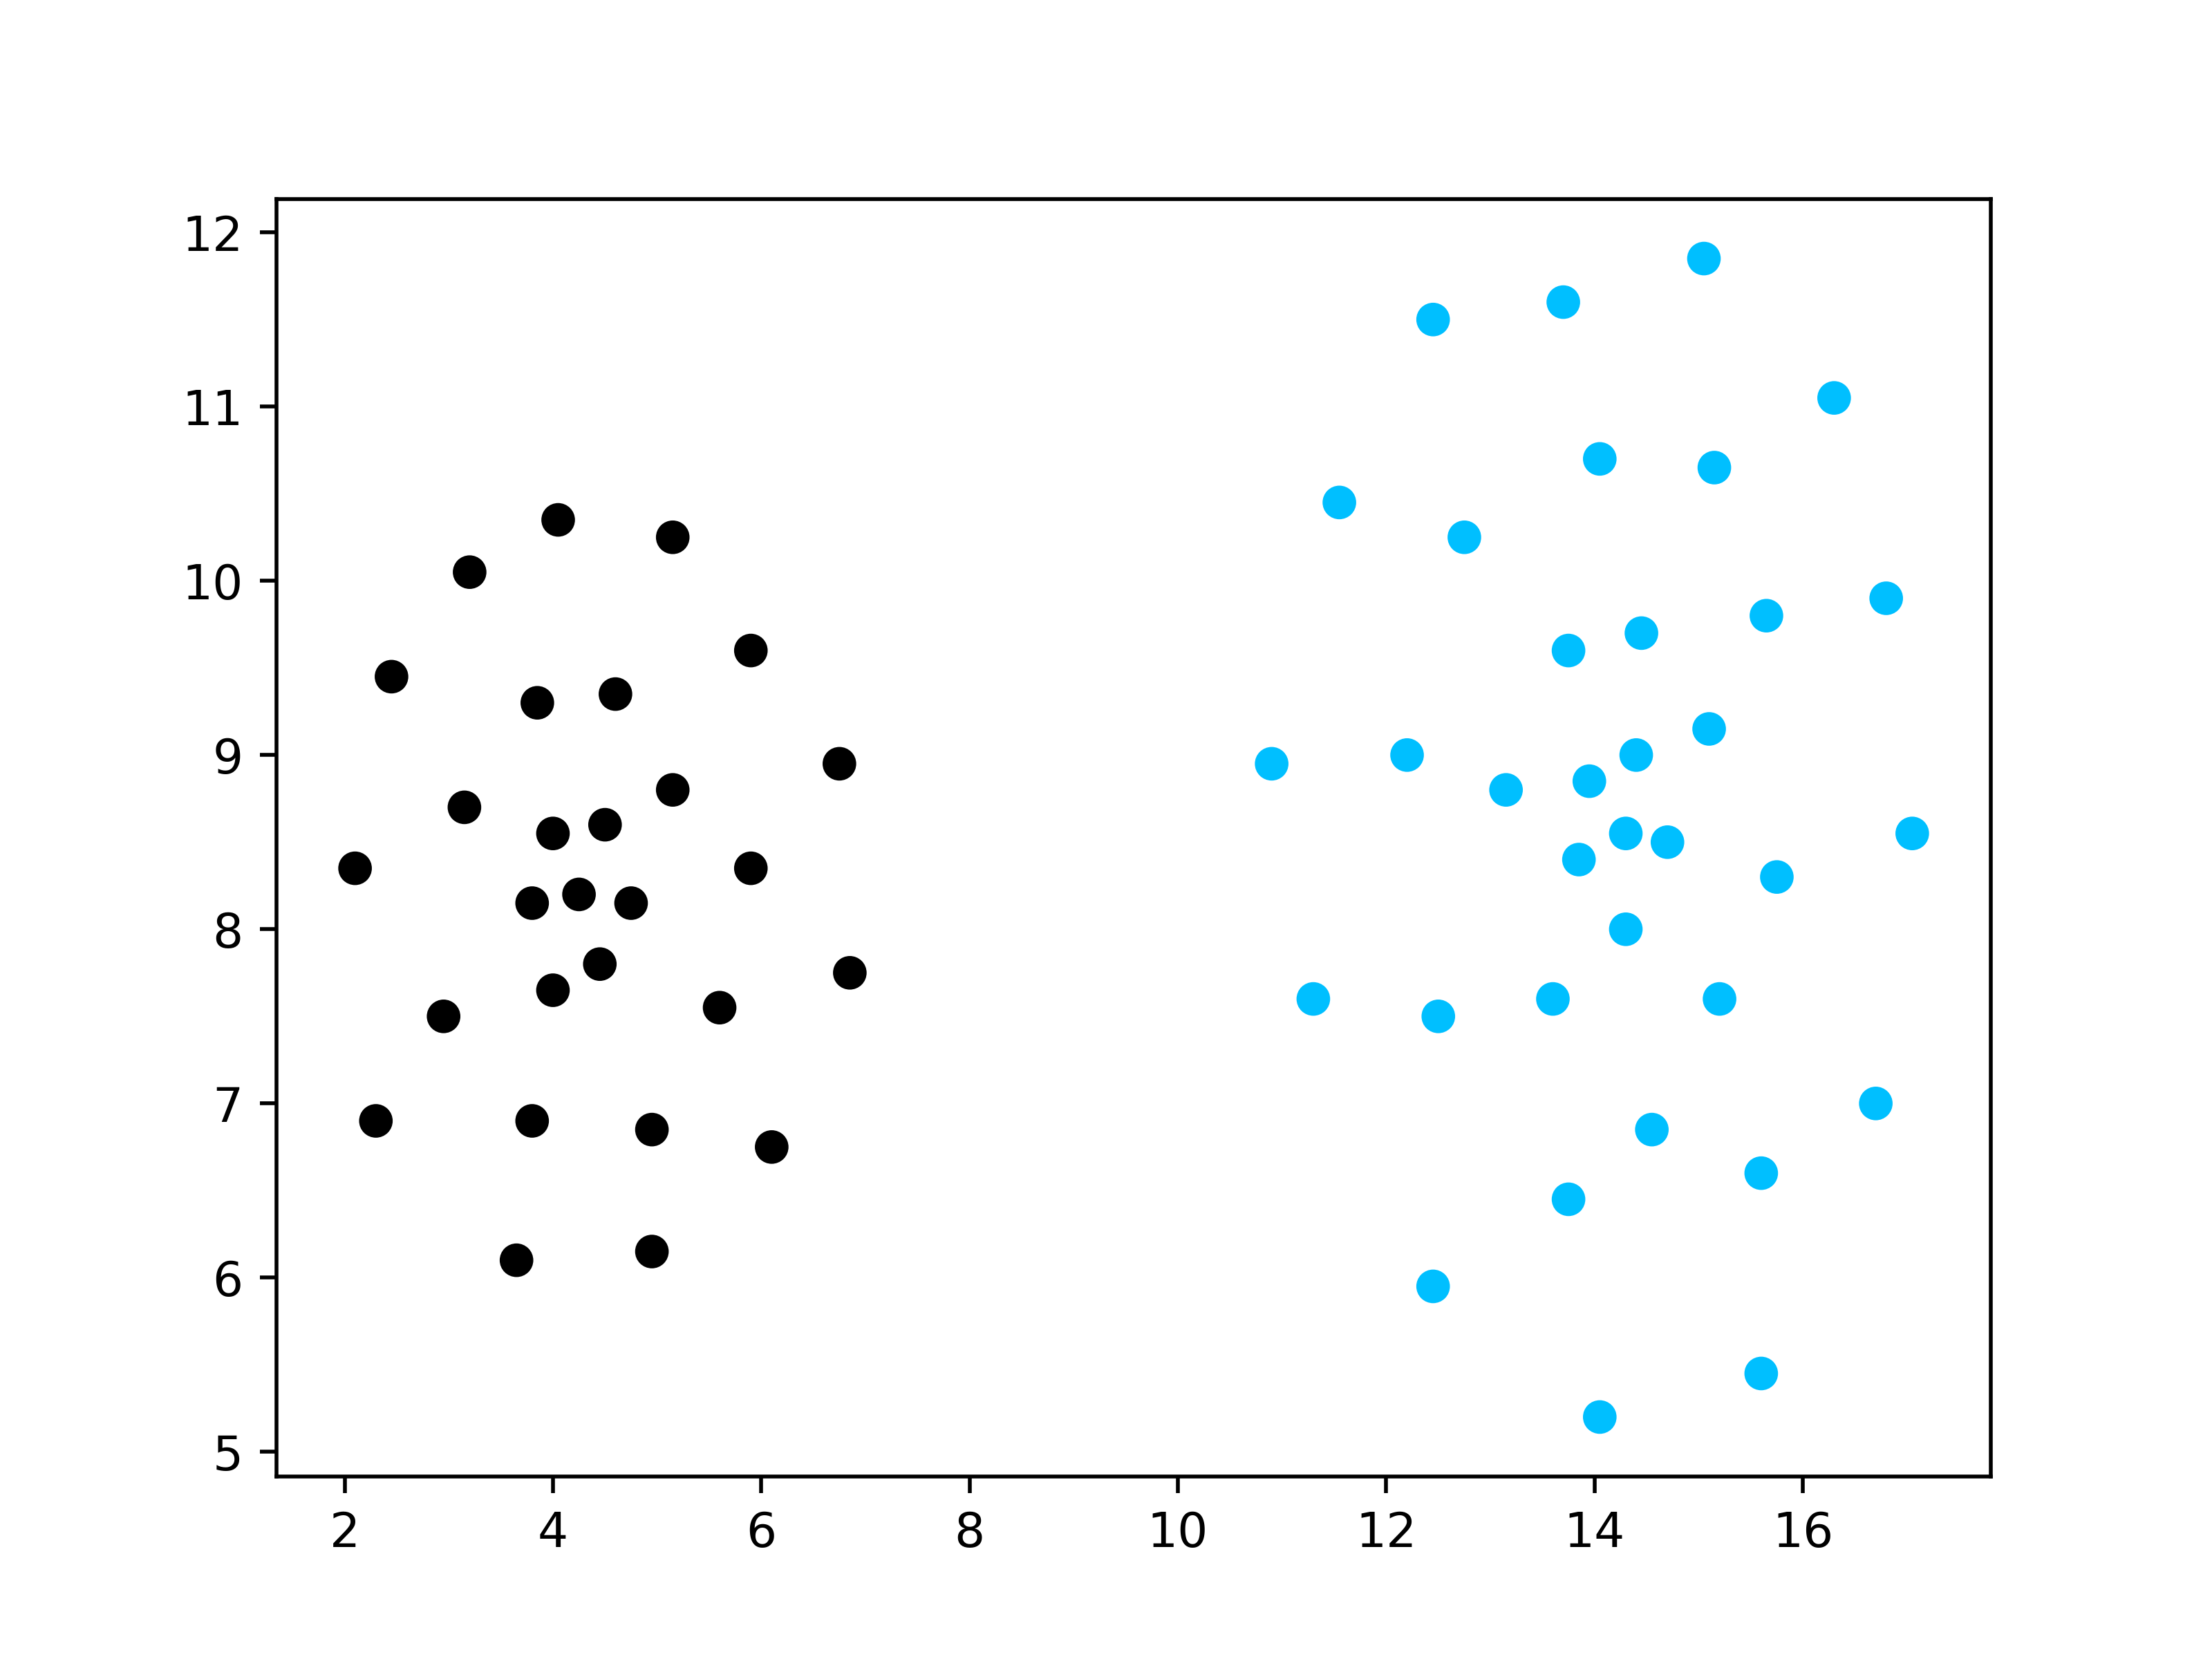
\includegraphics[width=0.43\linewidth]{our_gestalt_clusters.png}
	        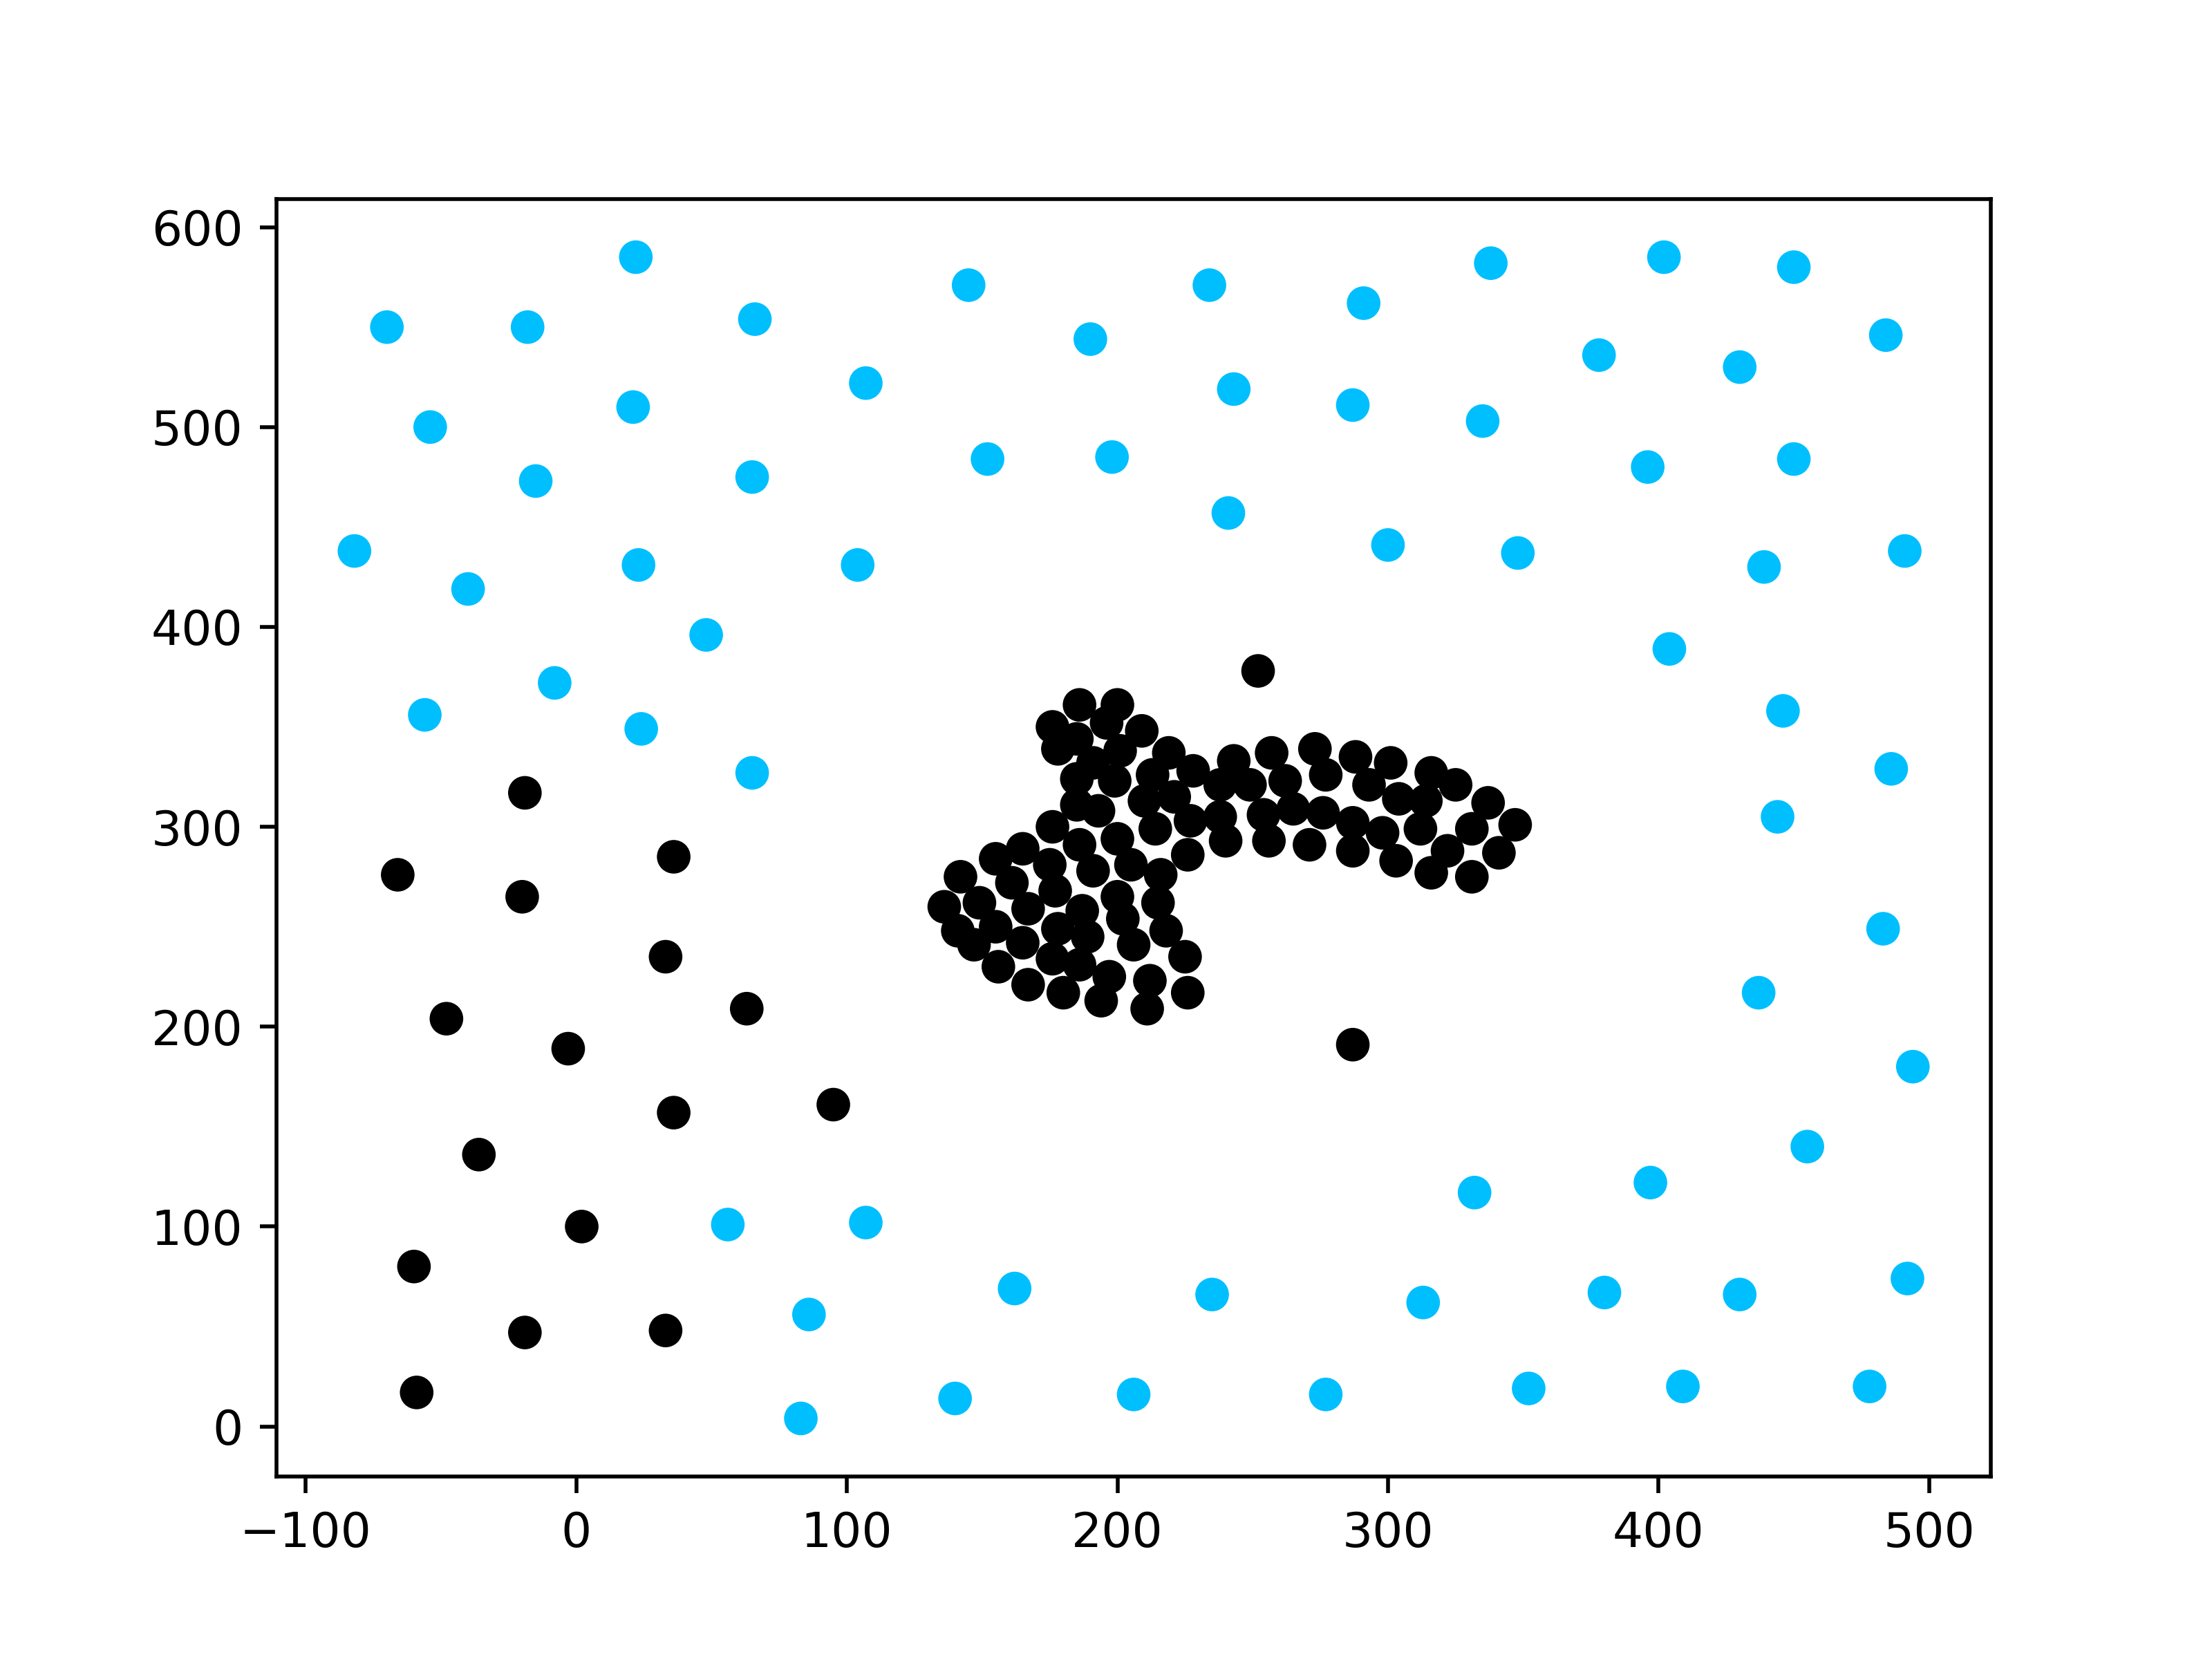
\includegraphics[width=0.43\linewidth]{our_h_clusters.png}
	        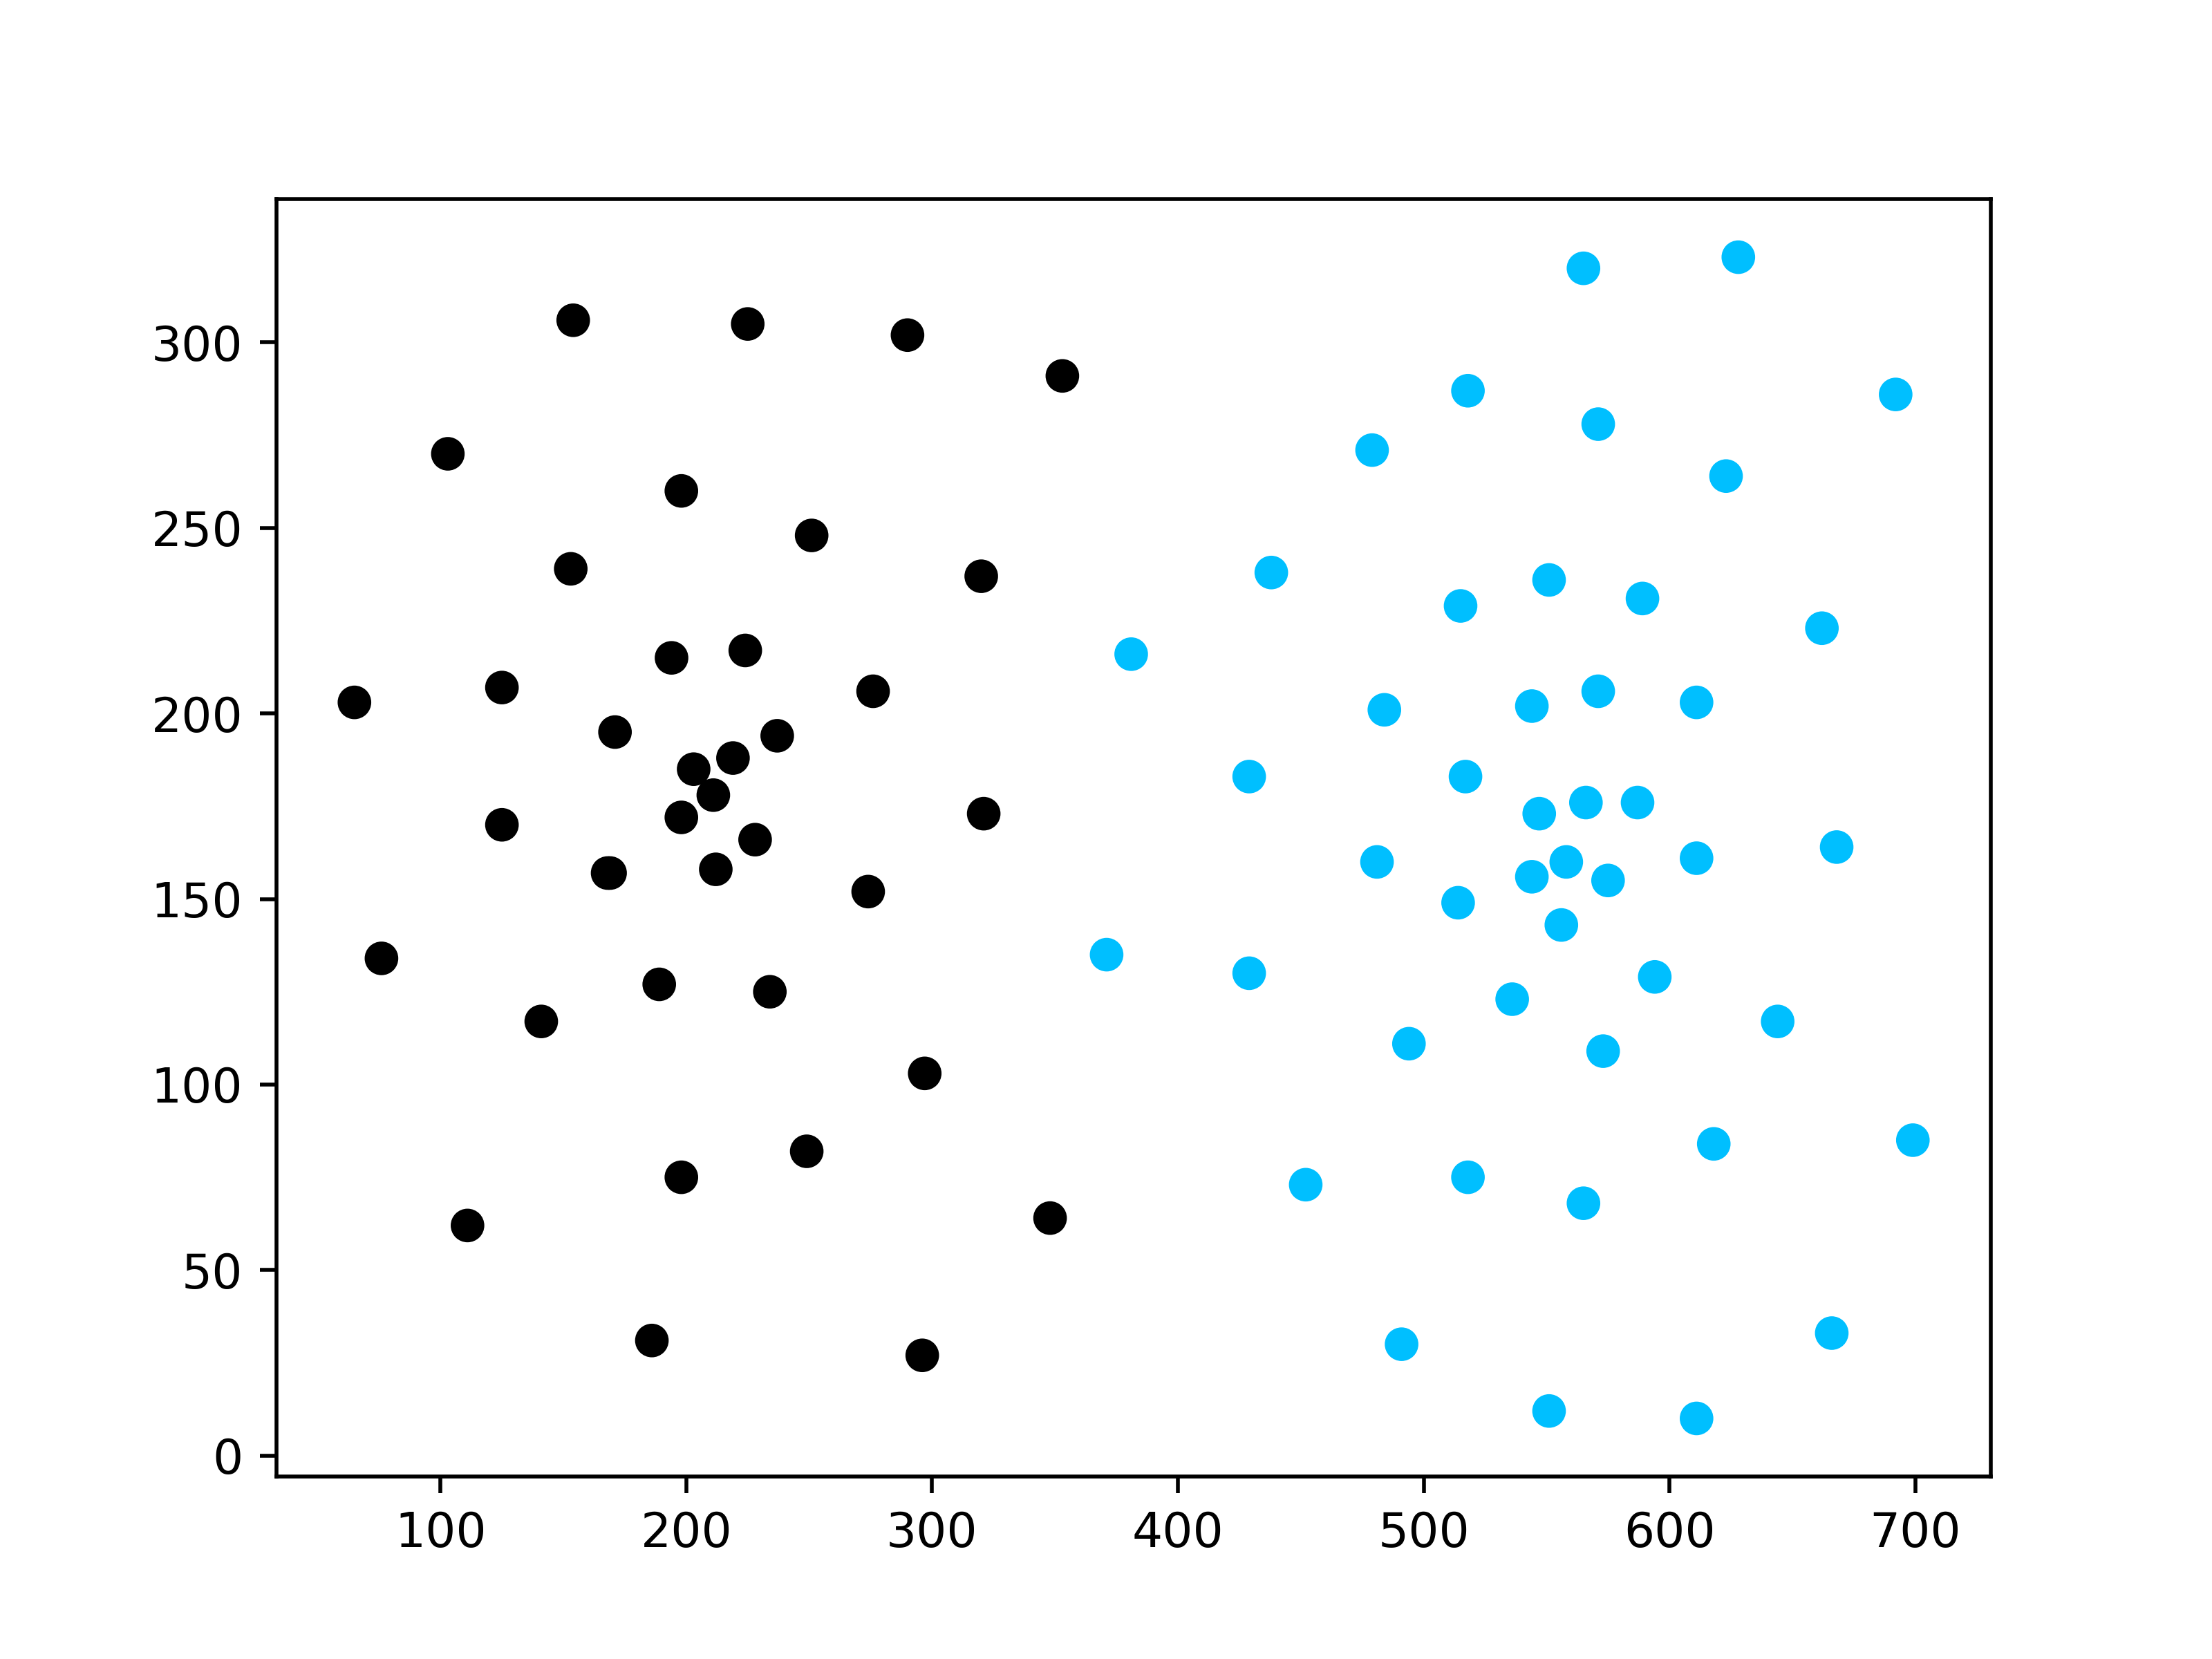
\includegraphics[width=0.43\linewidth]{our_i_clusters.png}
	        \caption{clustering results of our first Sampling-based MST algorithm}
	    \end{figure}

	    \begin{figure}[!t]
	        \centering
	        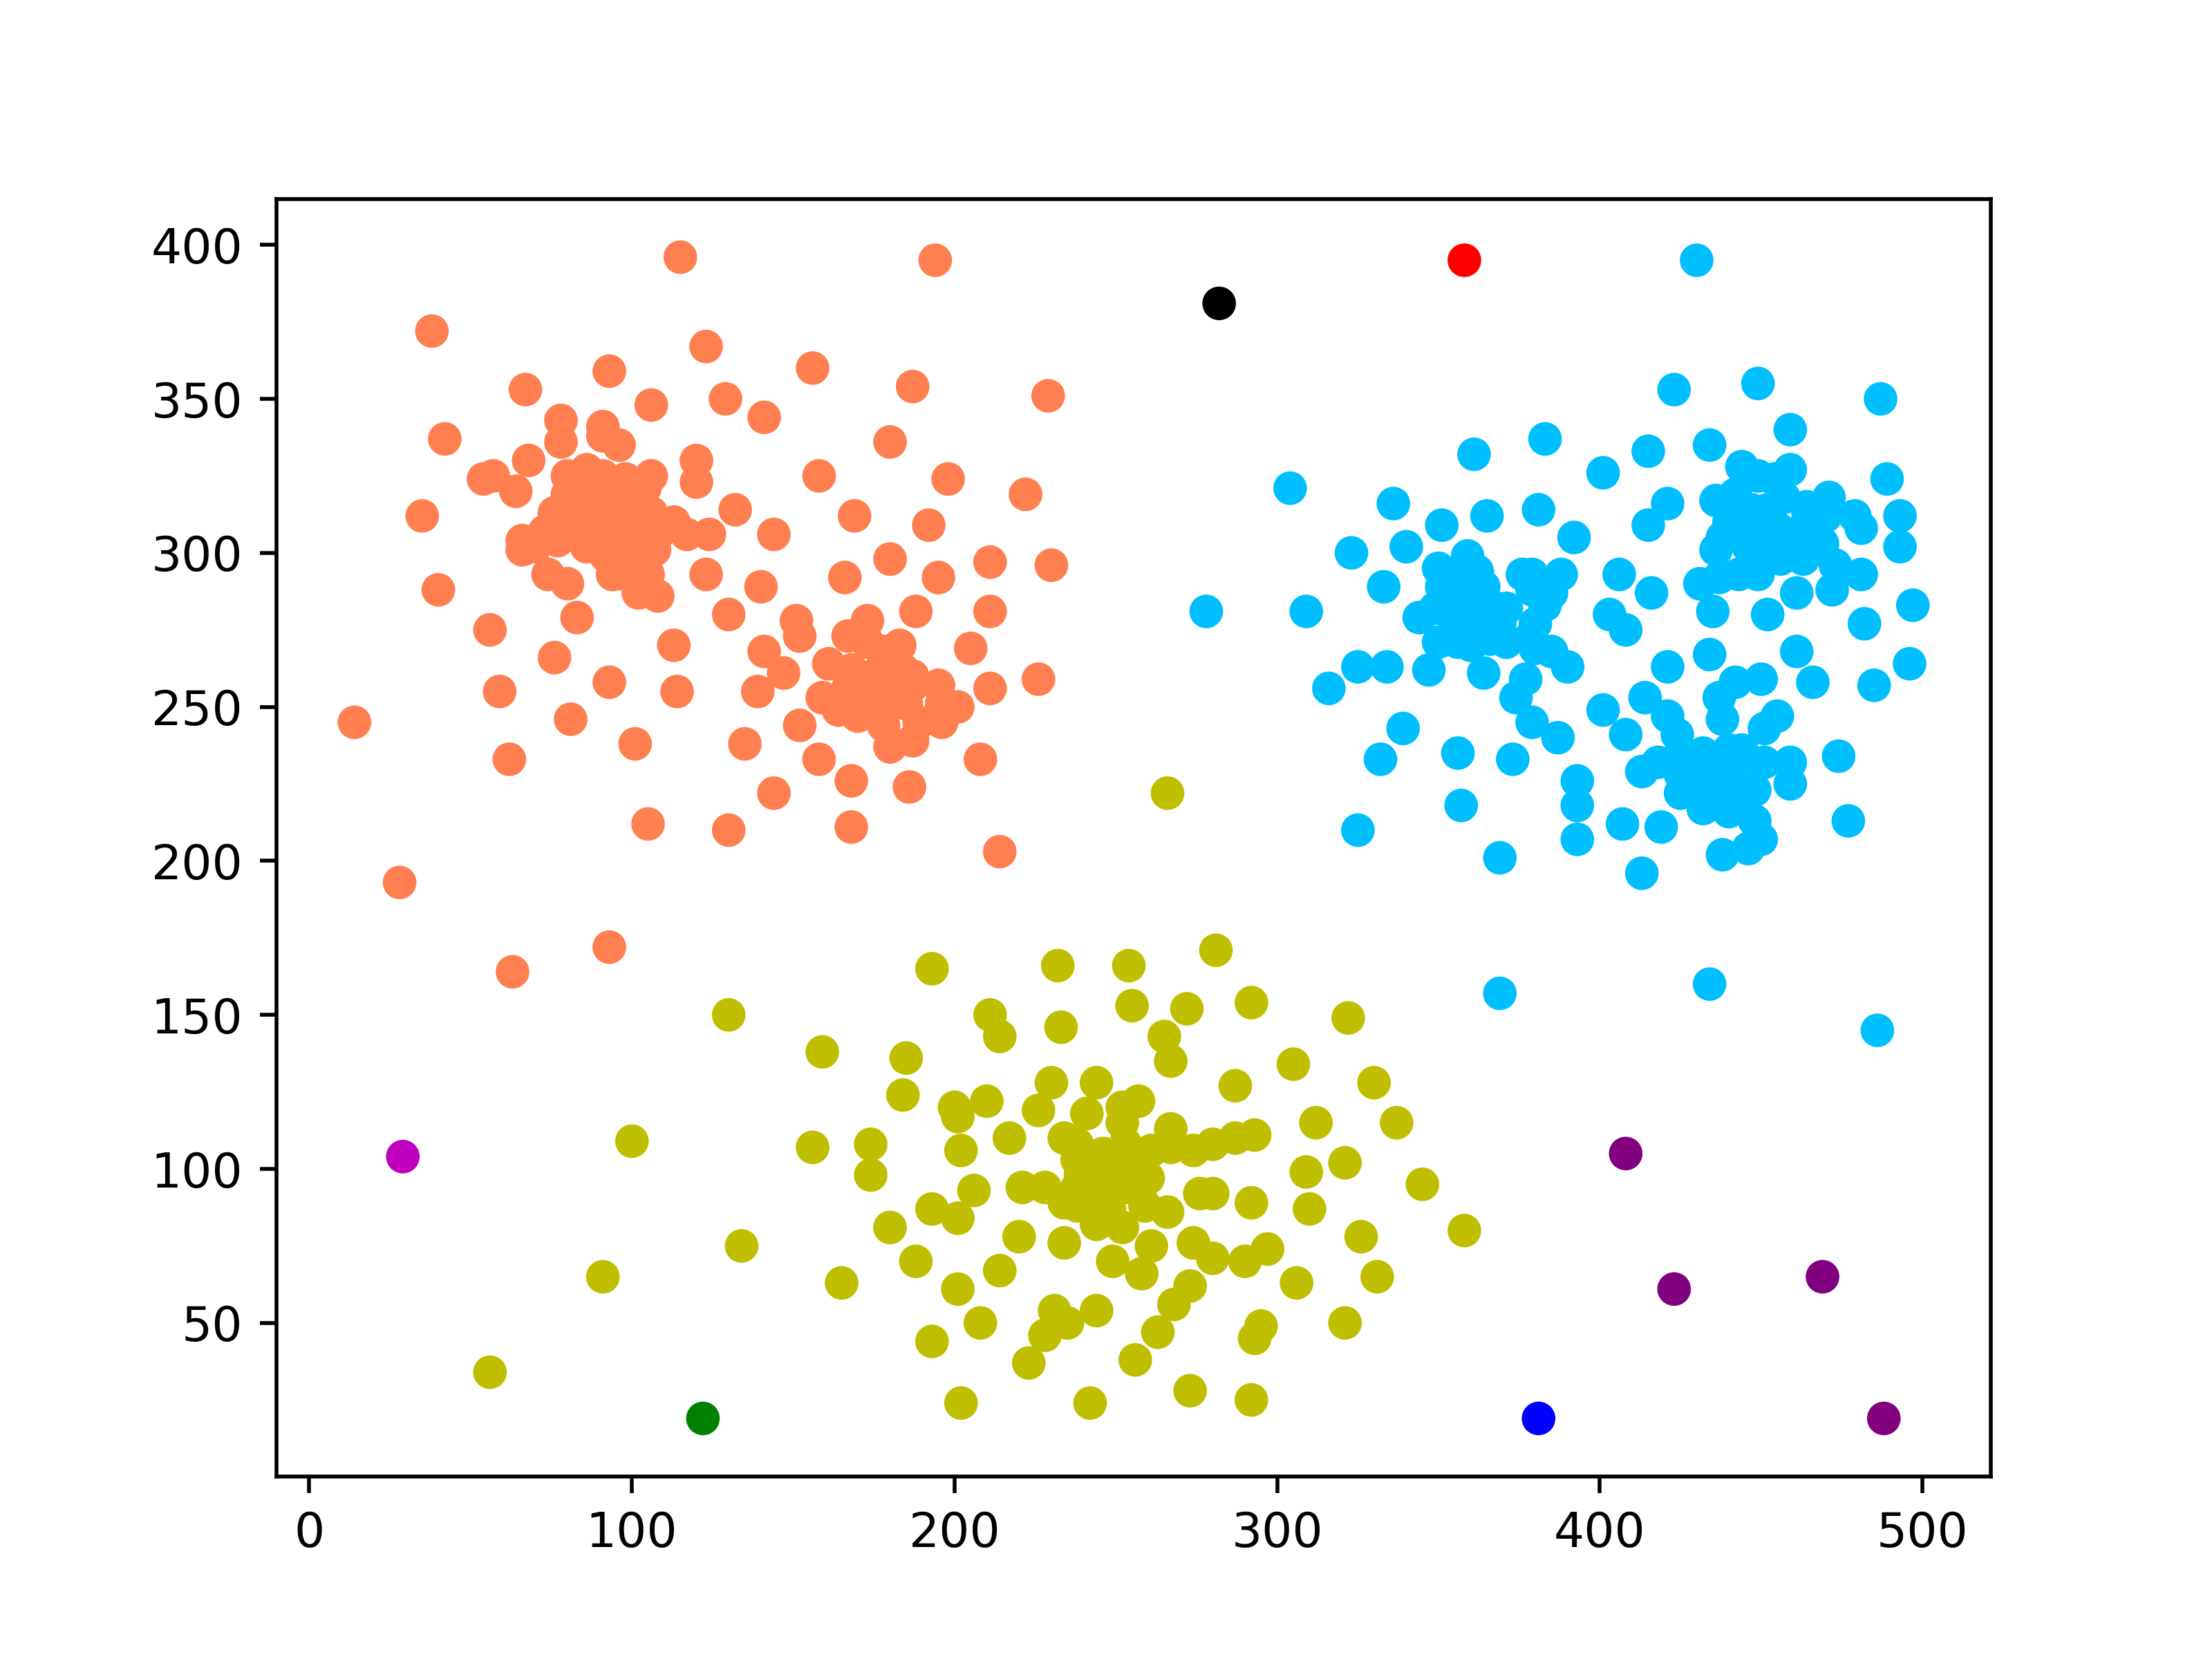
\includegraphics[width=0.43\linewidth]{our_ieee_clusters.png}
	        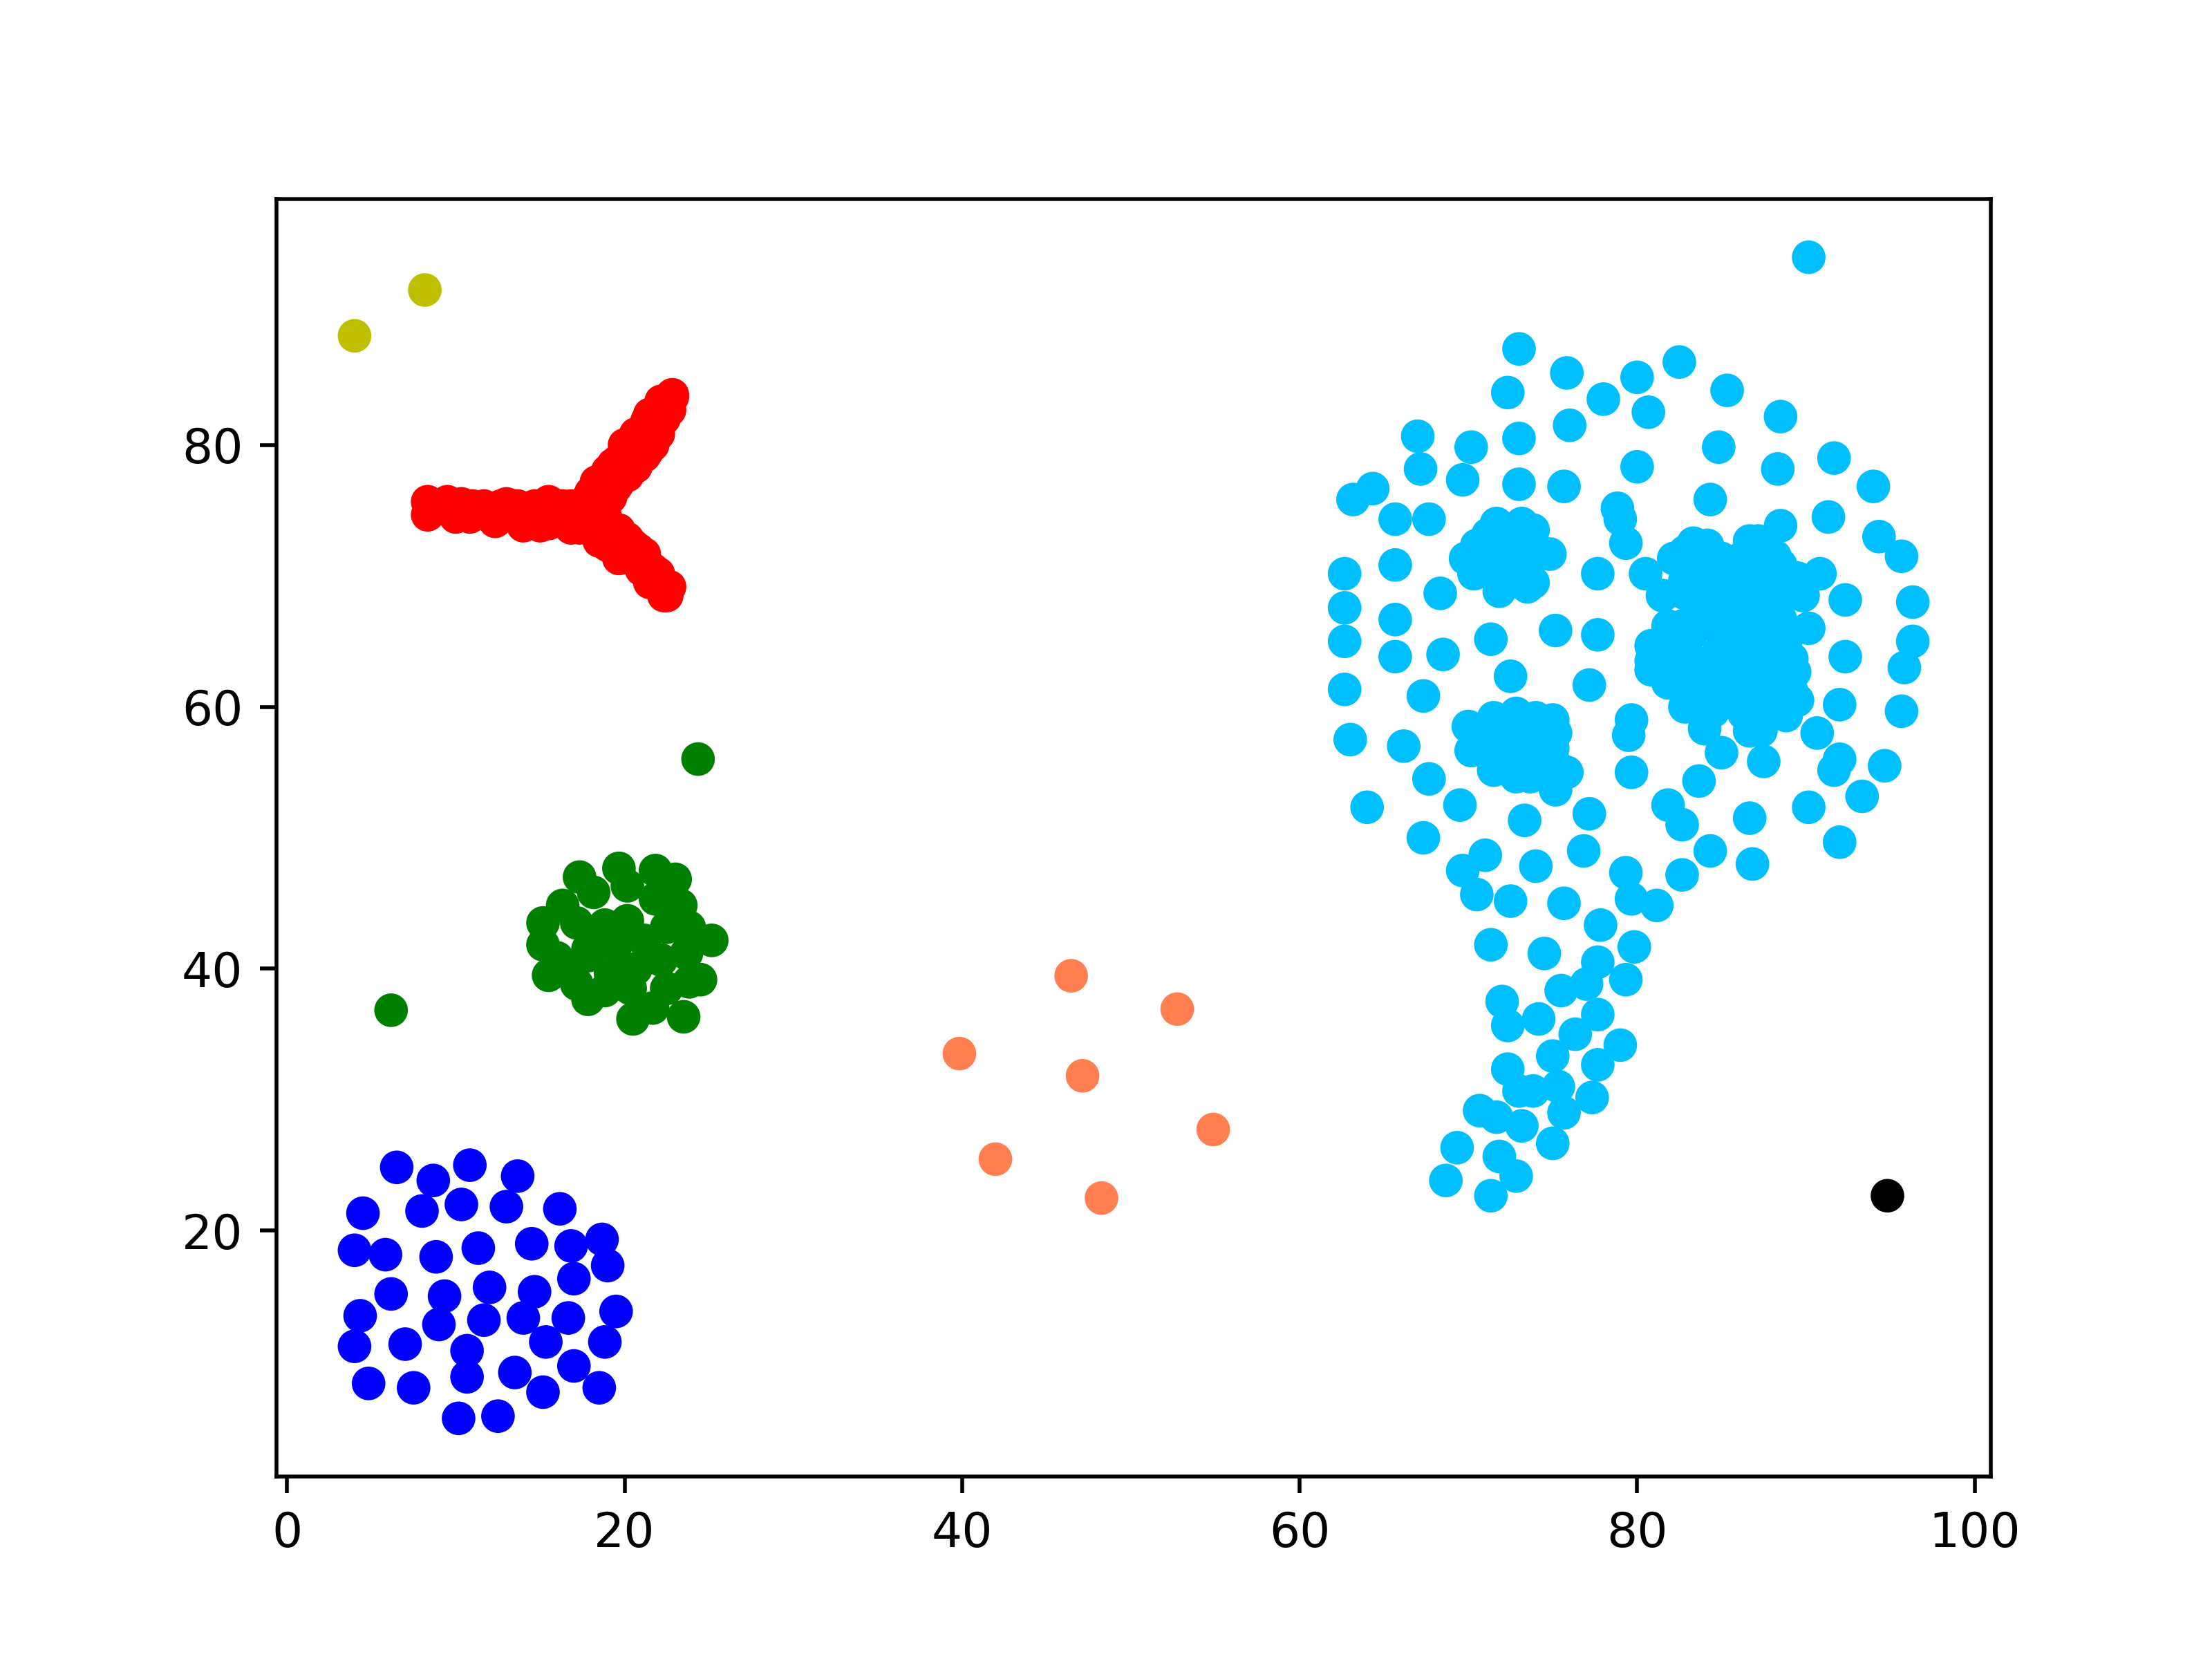
\includegraphics[width=0.43\linewidth]{our_l_clusters.png}
	        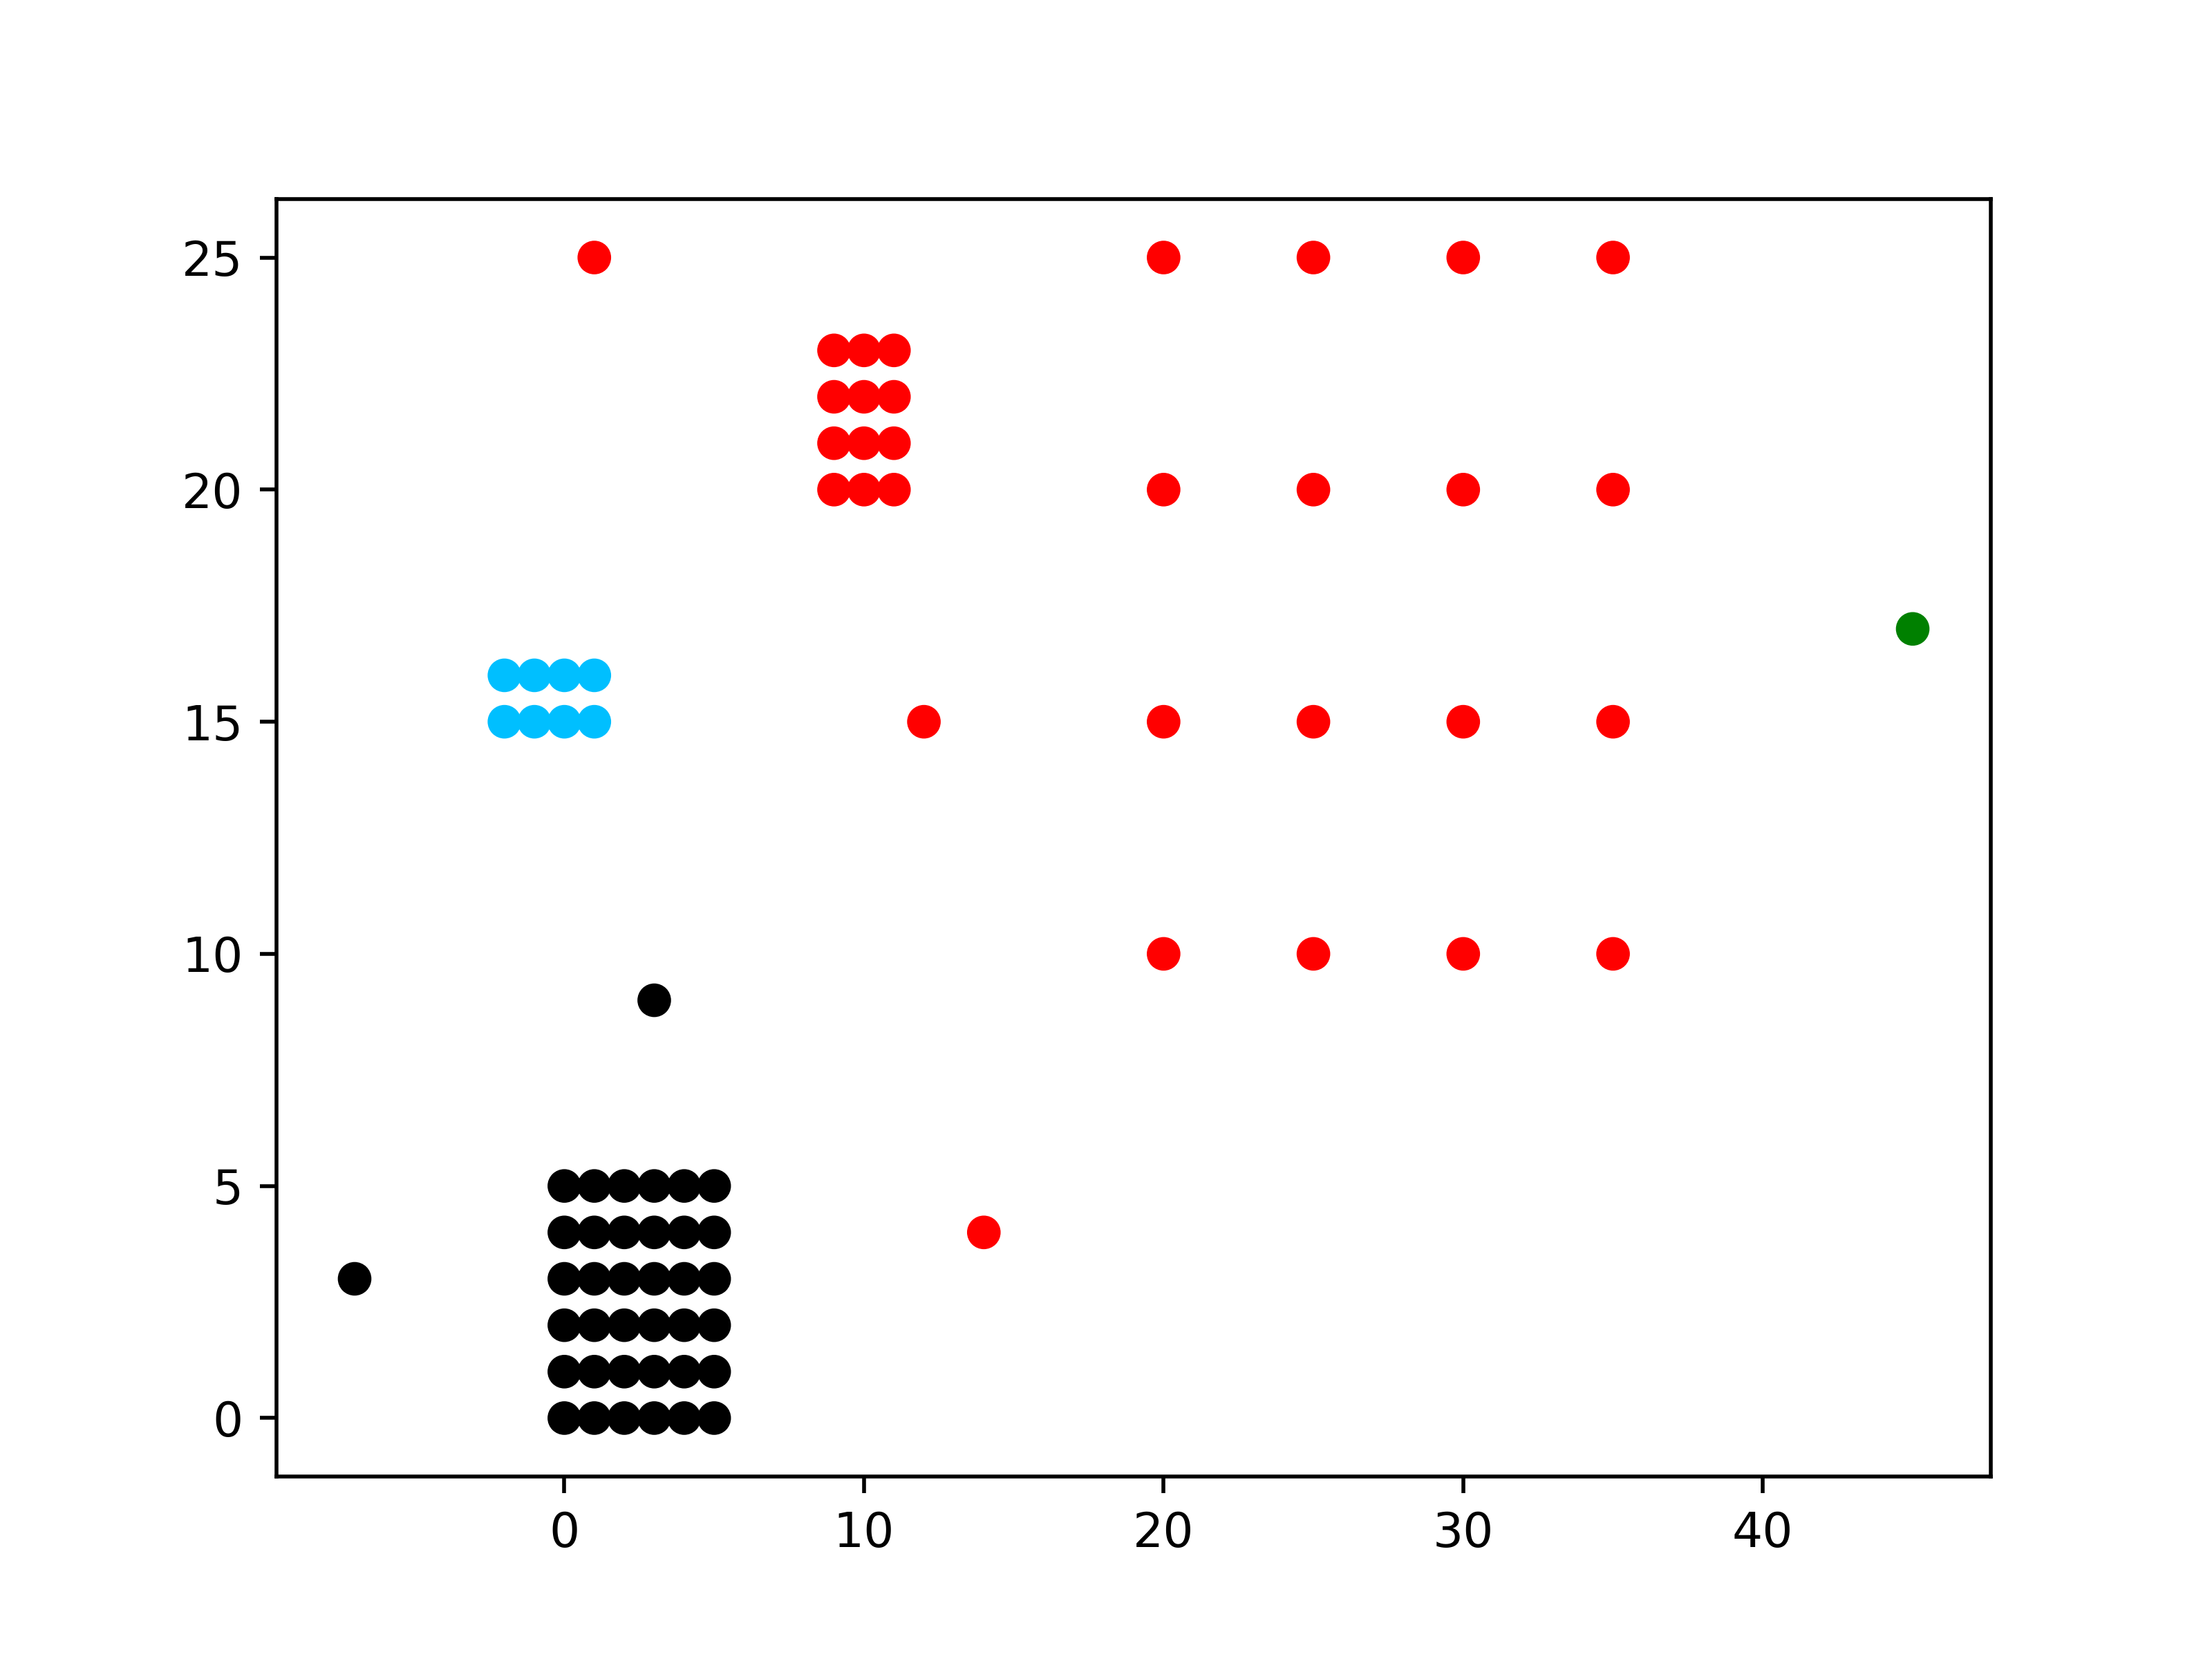
\includegraphics[width=0.43\linewidth]{our_syn1_2_clusters.png}
	        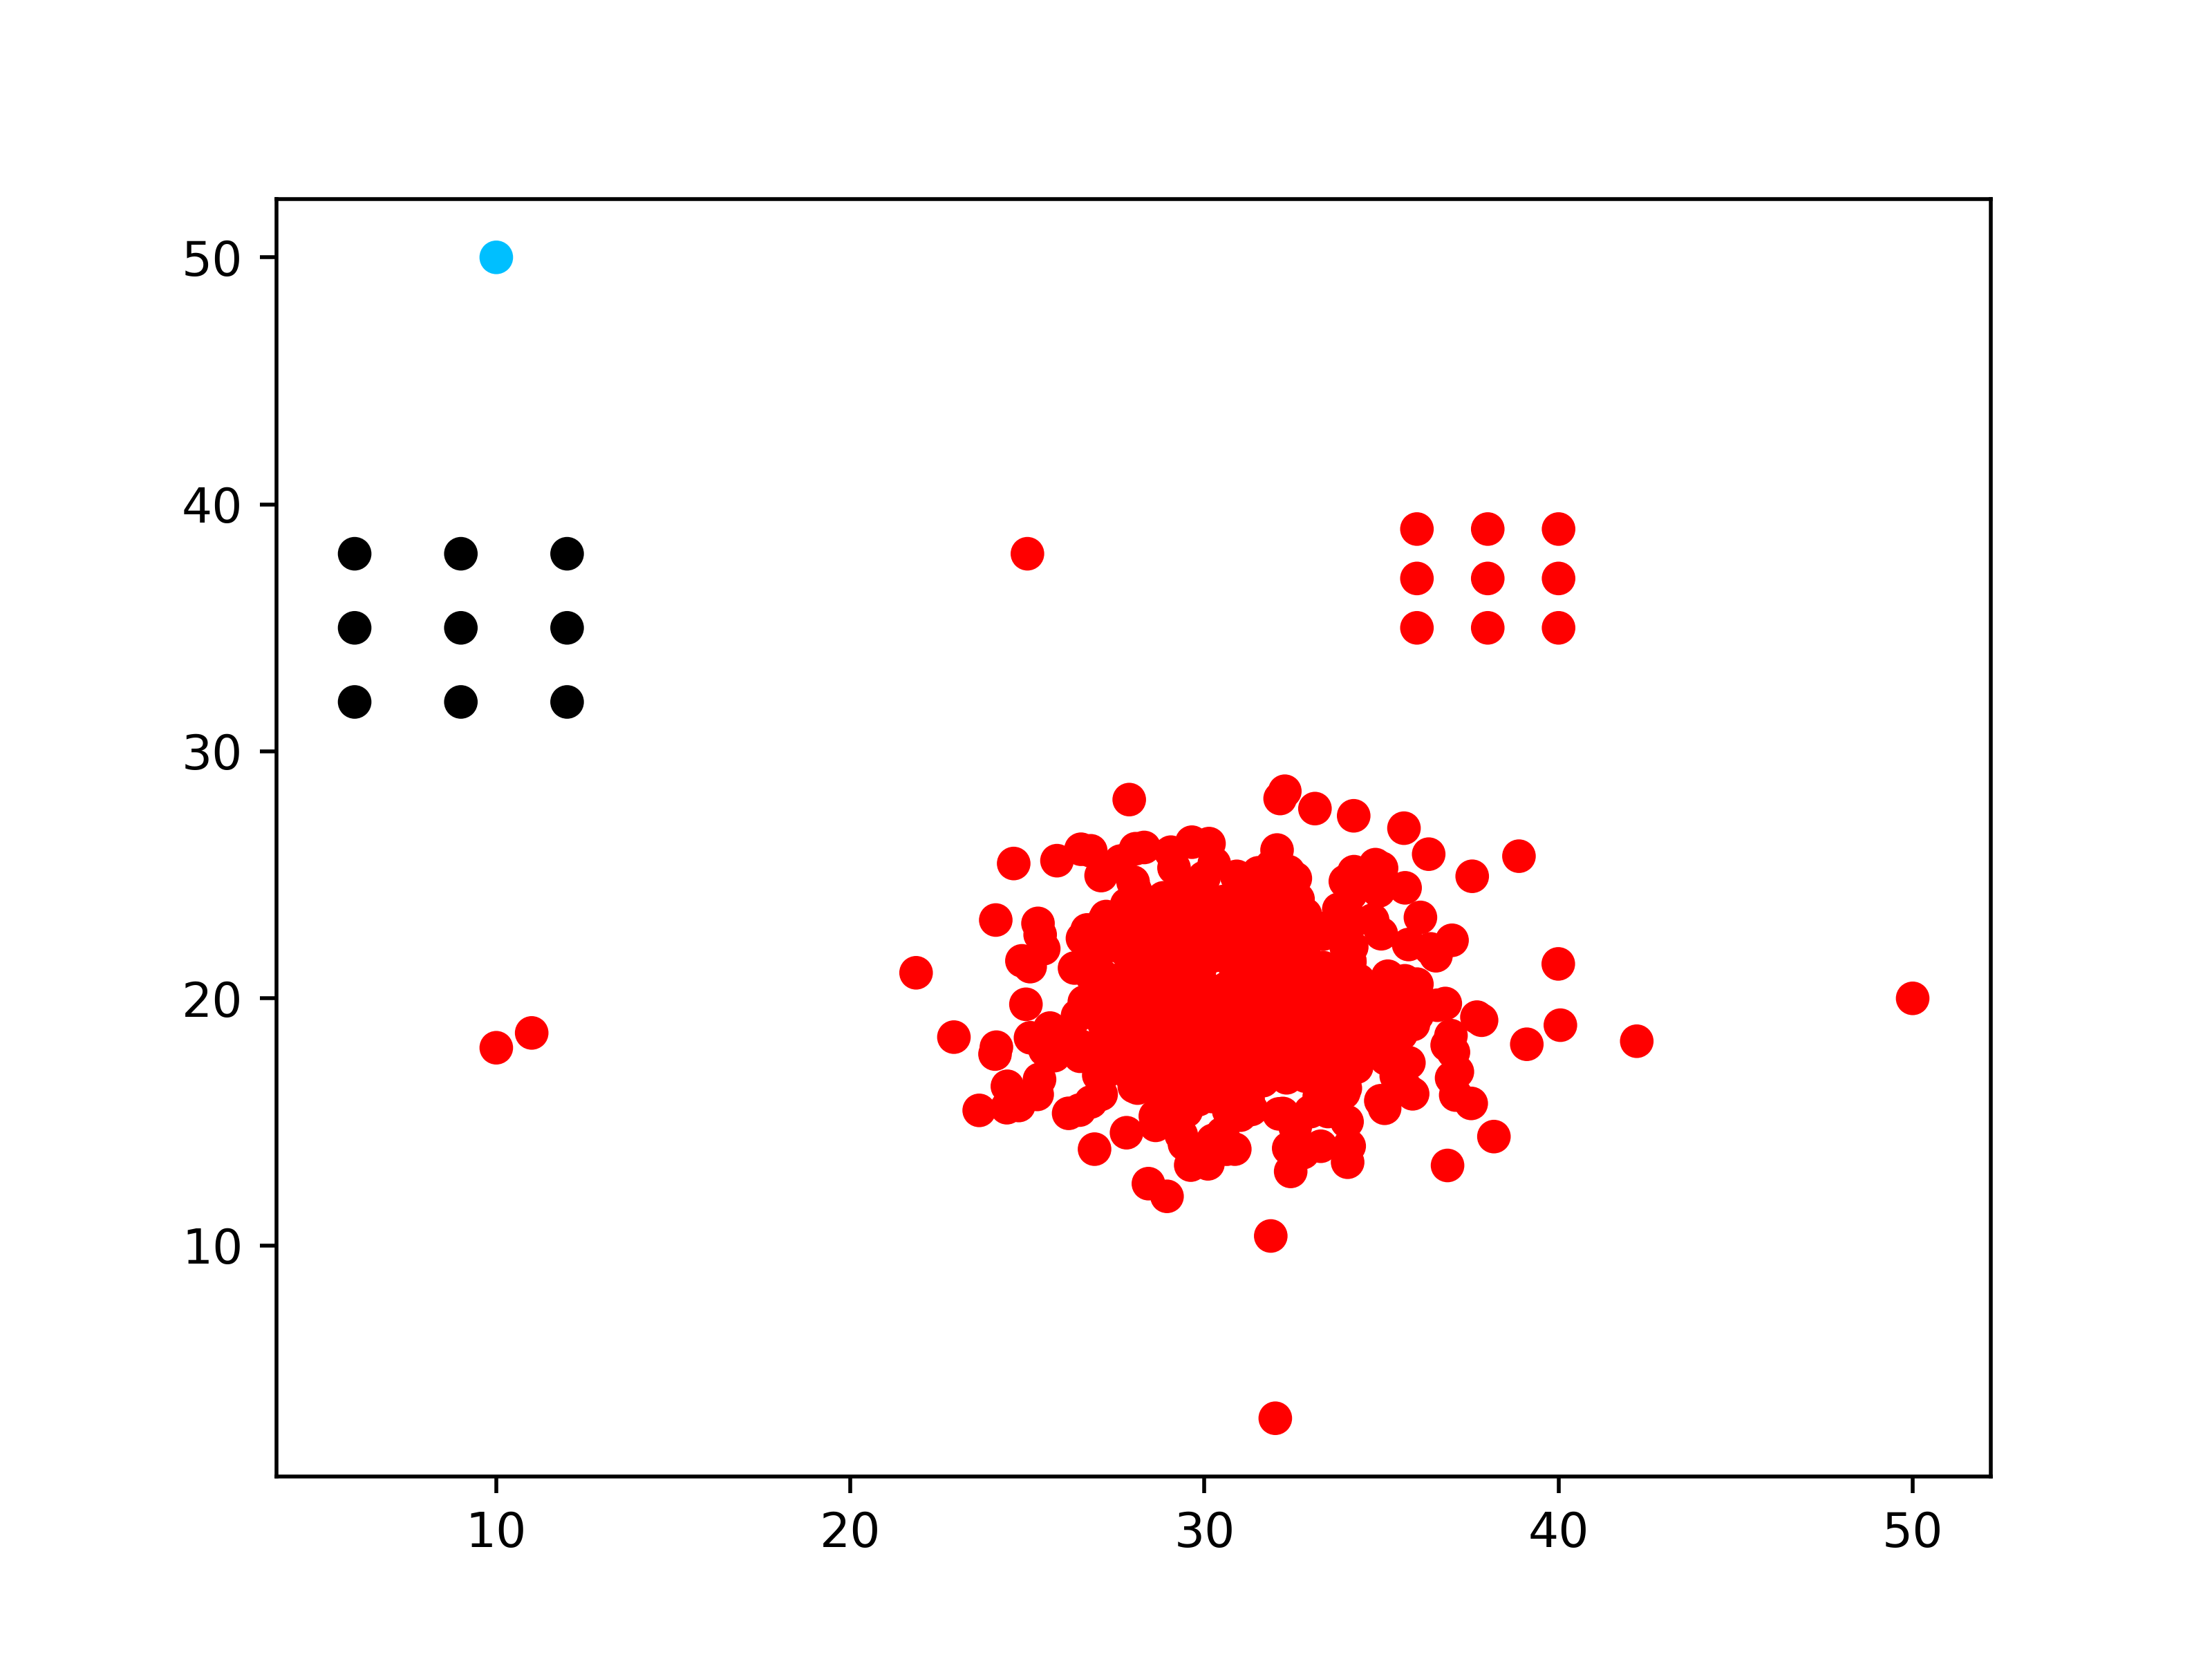
\includegraphics[width=0.43\linewidth]{our_syn2_1_clusters.png}
	        \caption{clustering results of our first Sampling-based MST algorithm}
	    \end{figure}

	\subsection{Results on real datasets}
		\begin{table}[htb]
	      \centering
	      \caption{description of data sets}
	      \label{my-label}
	      \begin{tabular}{|llll|}
	        \hline
	         Data Name & Size  & Attribute  & Class  \\ \hline
	         arcene 		& 200 	& 10000 & 2  \\ 
	         appendicitis 	& 106 	& 9 & 2 \\ 
	         banknote 		& 1372 	& 4 & 2 \\ 
	         breast cancer 	& 699 	& 9 & 2 \\ 
	         bupa 			& 345 	& 6 & 2 \\ 
	         fertility 		& 345 	& 7 & 2 \\ 
	         haberman 		& 306 	& 3 & 2 \\ 
	         hayes-roth 	& 160 	& 5 & 3 \\ 
	         ionosphere 	& 351 	& 33& 2 \\ 
	         iris 			& 150 	& 4 & 3 \\ 
	         newthyroid 	& 215 	& 5 & 3 \\ 
	         pima 			& 768 	& 8 & 2 \\ 
	         soybean-small 	& 47 	& 35& 4 \\ 
	         wdbc 			& 569 	& 30& 2 \\ 
	         wine 			& 178 	& 13& 3 \\ 
	         \hline
	      \end{tabular}
    	\end{table}

    	\begin{table}[htb]
	      \centering
	      \caption{Time cost on four algorithms}
	      \label{my-label}
	      \begin{tabular}{|llll|}
	        \hline
	         Data Name & kruscal  & FMST  & PNNG	& SMST\\ \hline
	         arcene 		&  51.13	& 	 & 281.22	& 19.88\\ 
	         appendicitis 	&  0.06	& 	 &	& \\ 
	         banknote 		&  6.80	& 	 &	& \\ 
	         breast cancer 	&  1.70	& 	 &	& \\ 
	         bupa 			&  0.38	& 	 &	& \\ 
	         fertility 		&  0.03	& 	 &	& \\ 
	         haberman 		&  0.26	& 	 &	& \\ 
	         hayes-roth 	&  0.06	& 	 &	& \\ 
	         ionosphere 	&  0.83	& 	 &	& \\ 
	         iris 			&  0.07	& 	 &	& \\ 
	         newthyroid 	&  0.12	& 	 &	& \\ 
	         pima 			&  2.20	& 	 &	& \\ 
	         soybean-small 	&  0.01	& 	 &	& \\ 
	         wdbc 			&  2.14 & 	 &	& \\ 
	         wine 			&  0.25 & 	 &	& \\ 
	         \hline
	      \end{tabular}
    	\end{table}

    	\begin{table}[htb]
	      \centering
	      \caption{clustering result of kruscal in different data sets}
	      \label{my-label}
	      \begin{tabular}{|lllll|}
	        \hline
	         Data Name & Rand Index  & Jaccard Index  & Adjust Rand Index & F\-measure  \\ \hline
	         arcene         & 0.5138 & 0.0266 & 0.3685 & 0.4041  \\ 
	         appendicitis   & 0.6679 & -0.0139 & 0.6667 & 0.8045 \\ 
	         banknote       & 0.5056 & -0.0002 & 0.5053 & 0.7100 \\ 
	         breast cancer  & 0.5484 & 0.0026 & 0.5476 & 0.7390\\ 
	         bupa           & 0.5104 & -0.0016 & 0.5091 & 0.7101  \\ 
	         fertility      & 0.7715 & -0.0164 & 0.7709 & 0.8661 \\ 
	         haberman       & 0.6126 & 0.0116 & 0.6107  & 0.7799  \\ 
	         hayes-roth     & 0.3742 & 0.0135 & 0.3613  & 0.5947 \\ 
	         ionosphere     & 0.5401 & 0.0045 & 0.5384  & 0.7317  \\ 
	         iris           & 0.7766 & 0.5638 & 0.5891  & 0.7535 \\ 
	         newthyroid     & 0.5441 & 0.0313 & 0.5367  & 0.7301  \\ 
	         pima           & 0.5458 & 0.0023 & 0.5451  & 0.7374 \\ 
	         soybean-small  & 0.8427 & 0.6537 & 0.6145  & 0.7839 \\ 
	         wdbc           & 0.5326 & 0.0024 & 0.5315  & 0.7277 \\ 
	         wine           & 0.3628 & 0.0054 & 0.3325  & 0.5431  \\ 
	         \hline
	      \end{tabular}
	    \end{table} 
		
		\begin{table}[htb]
	      \centering
	      \caption{clustering result of FMST in different data sets}
	      \label{my-label}
	      \begin{tabular}{|lllll|}
	        \hline
	         Data Name & Rand Index  & Jaccard Index  & Adjust Rand Index & F\-measure  \\ \hline
	         arcene         & 0.5138 & 0.0266 & 0.3685 & 0.4041  \\ 
	         appendicitis   &  & &  &  \\ 
	         banknote       &  & &  &  \\ 
	         breast cancer  &  & &  & \\ 
	         bupa           &  & &  &  \\ 
	         fertility      &  & &  & \\ 
	         haberman       &  & &  &  \\ 
	         hayes-roth     &  & &  & \\ 
	         ionosphere     &  & &  &  \\ 
	         iris           &  & &  & \\ 
	         newthyroid     &  & &  &  \\ 
	         pima           &  & &  & \\ 
	         soybean-small  &  & &  & \\ 
	         wdbc           &  & &  & \\ 
	         wine           &  & &  &  \\ 
	         \hline
	      \end{tabular}
	    \end{table} 

	    \begin{table}[htb]
	      \centering
	      \caption{clustering result of PNNG in different data sets}
	      \label{my-label}
	      \begin{tabular}{|lllll|}
	        \hline
	         Data Name & Rand Index  & Jaccard Index  & Adjust Rand Index & F\-measure  \\ \hline
	         arcene         & 0.5138 & 0.0266 & 0.3685 & 0.4041  \\ 
	         appendicitis   &  & &  &  \\ 
	         banknote       &  & &  &  \\ 
	         breast cancer  &  & &  & \\ 
	         bupa           &  & &  &  \\ 
	         fertility      &  & &  & \\ 
	         haberman       &  & &  &  \\ 
	         hayes-roth     &  & &  & \\ 
	         ionosphere     &  & &  &  \\ 
	         iris           &  & &  & \\ 
	         newthyroid     &  & &  &  \\ 
	         pima           &  & &  & \\ 
	         soybean-small  &  & &  & \\ 
	         wdbc           &  & &  & \\ 
	         wine           &  & &  &  \\ 
	         \hline
	      \end{tabular}
	    \end{table} 

	    \begin{table}[htb]
	      \centering
	      \caption{clustering result of SMST in different data sets}
	      \label{my-label}
	      \begin{tabular}{|lllll|}
	        \hline
	         Data Name & Rand Index  & Jaccard Index  & Adjust Rand Index & F\-measure  \\ \hline
	         arcene         & 0.5138 & 0.0266 & 0.3685 & 0.4041 \\ 
	         appendicitis   &  & &  &  \\ 
	         banknote       &  & &  &  \\ 
	         breast cancer  &  & &  & \\ 
	         bupa           &  & &  &  \\ 
	         fertility      &  & &  & \\ 
	         haberman       &  & &  &  \\ 
	         hayes-roth     &  & &  & \\ 
	         ionosphere     &  & &  &  \\ 
	         iris           &  & &  & \\ 
	         newthyroid     &  & &  &  \\ 
	         pima           &  & &  & \\ 
	         soybean-small  &  & &  & \\ 
	         wdbc           &  & &  & \\ 
	         wine           &  & &  &  \\ 
	         \hline
	      \end{tabular}
	    \end{table} 